\documentclass[a4paper]{article}

\usepackage{fullpage}
\usepackage{fancyhdr}
\usepackage{amsmath}
\usepackage{mathtools}
\usepackage{titling}
\usepackage{graphicx}
\usepackage{float}
\usepackage{multirow}
\usepackage{epsfig}
\usepackage[usenames]{color} 
\usepackage[export]{adjustbox}
\usepackage{enumitem}

\pagestyle{fancyplain}
\headheight 35pt
\rfoot{\small\thepage}
\headsep 1.5em

\begin{document}

\chead{{\Large{\bf PHYS414 Final Project}}} \lfoot{} \rfoot{\bf \thepage} \cfoot{} \rhead{\"{O}zg\"{u}r Bulut Karaosmano\u{g}u}

\section{Newton}

\begin{enumerate}[label=(\alph*)]
    \item We know that \\
    \begin{align}
        \frac{dm(r)}{dr} = 4\pi r^{2}\rho(r)\label{dmass}    \\
        \frac{dp(r)}{dr} = -\frac{Gm(r)\rho(r)}{r^{2}}\label{dpress}  \\
        p(r) = K{\rho(r)}^{1+\frac{1}{n}}\label{press} 
    \end{align}
    \eqref{dpress} can be rewritten as:
    \begin{equation}
      \frac{1}{\rho}\frac{dp}{dr} = -\frac{Gm}{r^{2}}
    \end{equation}
    Taking its derivative with respect to $r$ yields
    \begin{align}
        \frac{d}{dr}\left(\frac{1}{\rho}\frac{dp}{dr}\right) = \frac{2Gm}{r^{3}} - \frac{G}{r^{2}}\frac{dm}{dr}    \nonumber \\
        =-\frac{2}{r}\left(\frac{1}{\rho}\frac{dp}{dr}\right) - 4\pi G\rho \label{1/rhodpress}
    \end{align}
    By multiplying Eq.\eqref{1/rhodpress} with $r^{2}$, and collecting the $r$ derivatives of $p$ on one side, we get:
    \begin{align}
        \frac{d}{dr}\left(\frac{r^{2}}{\rho}\frac{dp}{dr}\right) = -4\pi Gr^{2}\rho \label{2nddevrho}
    \end{align}
     By introducing a new function $\theta$, which satisfies the relation $\rho = \rho_{c}\theta^{n}$($\rho_{c}$ is a constant), we can rewrite Eq.\eqref{press} as:
    \begin{equation}
        p = K  \rho_{c}^{1+\frac{1}{n}}\theta^{n+1} \label{newpress}
    \end{equation}
    Inserting Eq.\eqref{newpress} into \eqref{2nddevrho}, we get:
    \begin{equation}
        \frac{d}{dr}\left(\frac{r^{2}}{\rho_{c}\theta^{n}}K\rho_{c}^{\frac{1}{n} + 1}(n+1)\theta^{n} \frac{d\theta}{dr}\right) = -4G\pi r^{2}\rho_{c}\theta^{n}
    \end{equation}
    Simplified,
    \begin{equation}
        \frac{1}{r^{2}}\frac{d}{dr}\left(r^{2}K\rho_{c}^{\frac{1-n}{n}}(n+1)\frac{d\theta}{dr}\right) = -4G\pi \rho_{c}\theta^{n} \label{lastbeforefinal}
    \end{equation}
     By defining $\alpha \coloneqq \sqrt{K\rho_{c}^{\frac{1-n}{n}}(n+1)/4\pi G}$ and introducing a new variable $\xi$ which satisfies the relation $r = \alpha\xi$, we can rewrite Eq.\eqref{lastbeforefinal} as:
    \begin{equation}
        \frac{1}{\xi^{2}}\frac{d}{d\xi} \left(\xi^{2}\frac{d\theta}{d\xi}\right) + \theta^{n} = 0 \label{laneemden}
    \end{equation}
    which is the Lane-Emden equation.
    
    Analytical solutions of Lane-Emden equation only exist for $n=0,1,5$. The regular solutions near the center, i.e. $\xi\approx 0$ can be approximated as a power series:
    \begin{equation}
        \theta(\xi) = 1 - \frac{1}{6}\xi^{2} + \frac{n}{120}\xi^{4} + \dots
    \end{equation}
    This series has an error of order $O(\xi^{6})$.
    
    The Mathematica code used to calculate this series expression can be found in the Supplementary Material.
    
    Eq.\eqref{dmass} can be rewritten as
    \begin{equation}
        dm(r) = 4\pi r^{2}\rho(r)dr \label{dmassnew}
    \end{equation}
    which, after scaling the appropriate variables ($\rho = \rho_{c}$ , $r = \alpha\xi$), becomes
    \begin{equation}
        dm = 4\pi \rho_{c} \alpha^{3}\xi^{2} \theta^{n}d\xi 
    \end{equation}
    Integrating both sides from $0$ to $\xi_{n}$ gives
    \begin{align}
        m = 4\pi \rho_{c} \alpha^{3} \int_{0}^{\xi_{n}} \xi^{2} \theta^{n}d\xi \nonumber \\
          = 4\pi \rho_{c} \alpha^{3} \int_{0}^{\xi_{n}} -\frac{d}{d\xi} \left(\xi^{2}\frac{d\theta}{d\xi}\right) d\xi \nonumber \\
        = 4\pi \rho_{c} \alpha^{3}\xi_{n}^{2} \left(-\theta '(\xi_{n}) \right) \label{mass}
    \end{align}
    Since $r = \alpha\xi$ and $\xi_{n}$ is the maximum value of $\xi$ where $\theta(\xi) \geq 0$, we can conclude that $R = \alpha\xi_{n}$ is the radius of the star. Multiplying and dividing Eq.\eqref{mass} with $\xi_{n}$ to write it in terms of $R$, we get:
    \begin{equation}
        M = 4\pi \rho_{c} R^{3} \left(-\frac{\theta '(\xi_{n})}{\xi_{n}} \right)
    \end{equation}
    In order to find the total mass of a star in terms of its radius, we need to combine Eq.\eqref{mass} and $R = \alpha\xi_{n}$.
    
    We'll get rid of $\alpha$, and write its true value instead, with the aim to connect the two equations by isolating $\rho_{c}$ in each one. Eq.\eqref{mass}, with this prescription, can be written as:
    \begin{equation}
        M = 4\pi \left(\frac{K(n+1)}{4\pi G}\right)^{\frac{3}{2}} \left(-\xi_{n}^{2}\theta '(\xi_{n})\right) \rho_{c}^{\frac{3-n}{2n}}
    \end{equation}
    Similarly, 
    \begin{equation}
        R = \alpha\xi_{n} = \left(\frac{K(n+1)}{4\pi G}\right)^{\frac{1}{2}} \xi_{n} \rho_{c}^{\frac{1-n}{2n}}
    \end{equation}
    Isolating $\rho_{c}$ form both equations, we get:
    \begin{align}
        \rho_{c} = \left( \frac{M}{4\pi \left(\frac{K(n+1)}{4\pi G}\right)^{\frac{3}{2}} \left(-\xi_{n}^{2}\theta '(\xi_{n})\right)} \right)^{\frac{2n}{3-n}}     \nonumber \\
        = \left( \frac{R}{\left(\frac{K(n+1)}{4\pi G}\right)^{\frac{1}{2}} \xi_{n}} \right)^{\frac{2n}{1-n}}
    \end{align}
    which results in the relation:
    \begin{equation}
        M = (4\pi)^{\frac{1}{1-n}} \left(\frac{K(n+1)}{G}\right)^{\frac{n}{n-1}} \xi_{n}^{\frac{n+1}{n-1}} (-\theta '(\xi_{n}) ) R^{\frac{3-n}{1-n}}
    \end{equation}

  \item The Python code for extracting the $.csv$ file can be found in the Supplementary Material. The $M$ vs $R$ plot of the white dwarfs is included in Figure 1.
    \begin{figure}[H] 
    \centering
    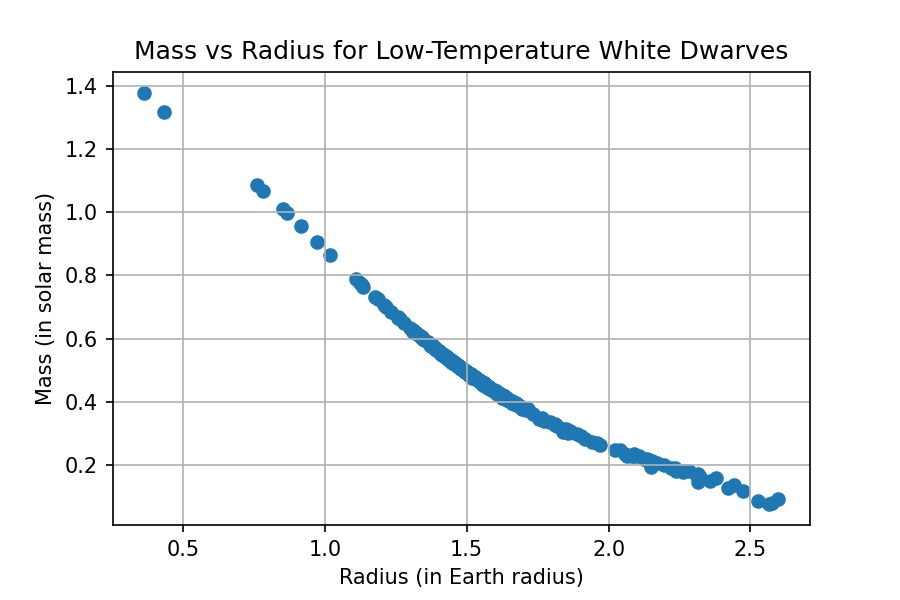
\includegraphics[width=0.85\textwidth]{WD.jpg}
    \caption{Mass v Radius plot of low-temperature White Dwarves.}
    \end{figure}

    \item The series expansion (obtained by Mathematica) for the polytropic approximation of pressure is:
    \begin{align}
        P = \frac{Cx^{5}}{5} + \mathcal{O}(x^{6}) \nonumber \\
        \simeq \frac{8C}{5D^{{5} / {q}}} \rho^{1 + \frac{1}{{q} / {(5-q)}}}
    \end{align}
    which yields the constants $K_{*}$ and $n_{*}$.
    
    After making the appropriate fit, $q$ seems to be fluctuating around $3$, as seen in Figure 2. Since we know from theory that $q$ is an integer, we can deduce that $q$ is exactly equal to 3.
    \begin{figure}[H] 
    \centering
    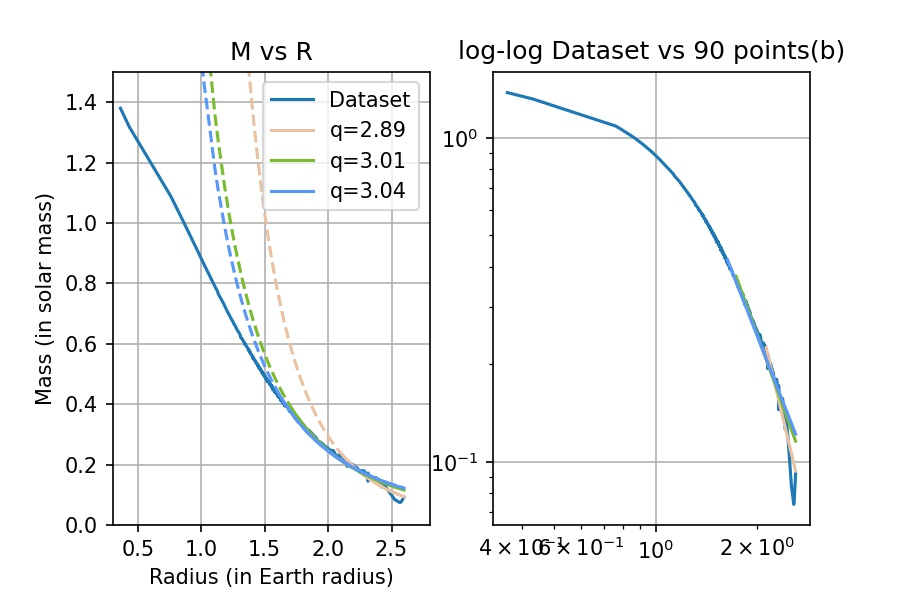
\includegraphics[width=0.85\textwidth]{WD_loglog.jpg}
    \caption{a) M-R plot, low-mass fit. b) log-log plots.}
    \end{figure}
    
    After obtaining the specific value of $q$, and subsequently $n_{*}$, another fitting reveals the value of $K_{*}$, which turns out to be $\approx 2.83 \times 10^{12}$ cm$^{4}$ g$^{-\frac{2}{3}}$ s$^{-2}$. 
    
    \begin{figure}[H] 
    \centering
    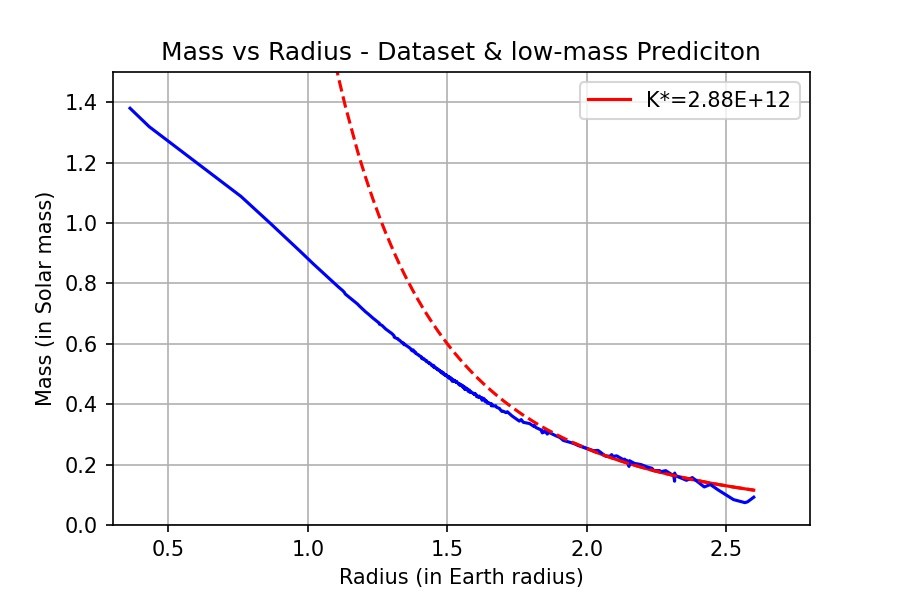
\includegraphics[width=0.85\textwidth]{WD_DatvPrd.jpg}
    \caption{M-R plot and $K_{*}$ fit}
    \end{figure}
    
    Central density $\rho_{c}$ has the formula:
    \begin{equation}
        \rho_{c} = \frac{M}{4\pi R^{3}} \frac{\xi_{n}^{3}}{\left(-\xi^{2} \theta'(\xi)\right)_{\xi=\xi_{n}}}
    \end{equation}
    
    $\xi_{n}$ and $\left(-\xi^{2} \theta'(\xi)\right)_{\xi=\xi_{n}}$ can be obtained by solving the Lane-Emden Equation. After substituting the appropriate values, we find $\rho_{c}$ to be proportional to $M^2$, which can be seen in Figure 4.
    
    \begin{figure}[h] 
    \centering
    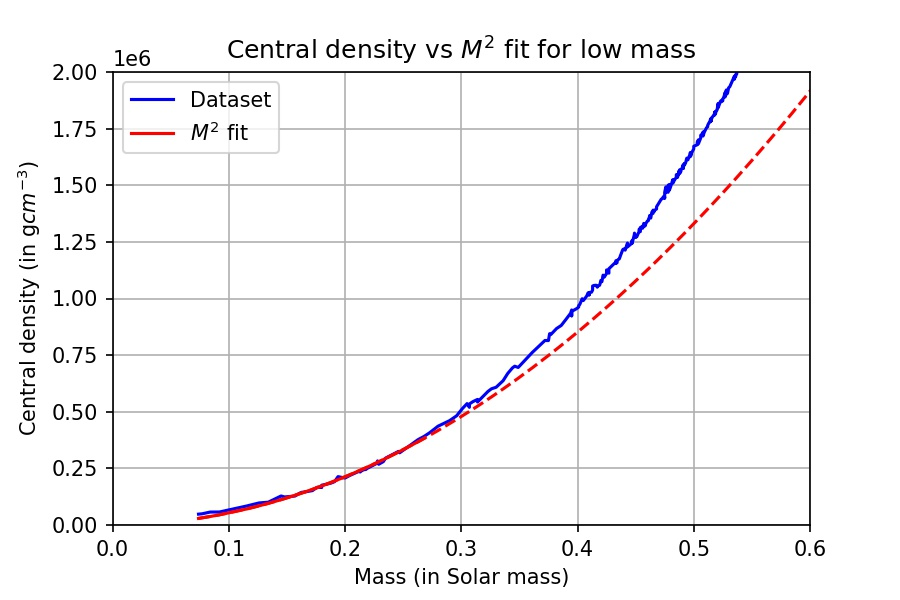
\includegraphics[width=0.85\textwidth]{WD_Dense.jpg}
    \caption{Density vs Mass, $M^2$ fit (red)}
    \end{figure}  

 \item A range of $(10^{5}, 10^{9})$ was used for  $\rho_{c}$ and possible $D$ values between $(10^{6}, 10^{7})$. The $D$ value with lowest RMS error approximated the theoretical value $D = 2.00 \times 10^{6}$, which was thus used.
    
    \begin{figure}[H] 
    \centering
    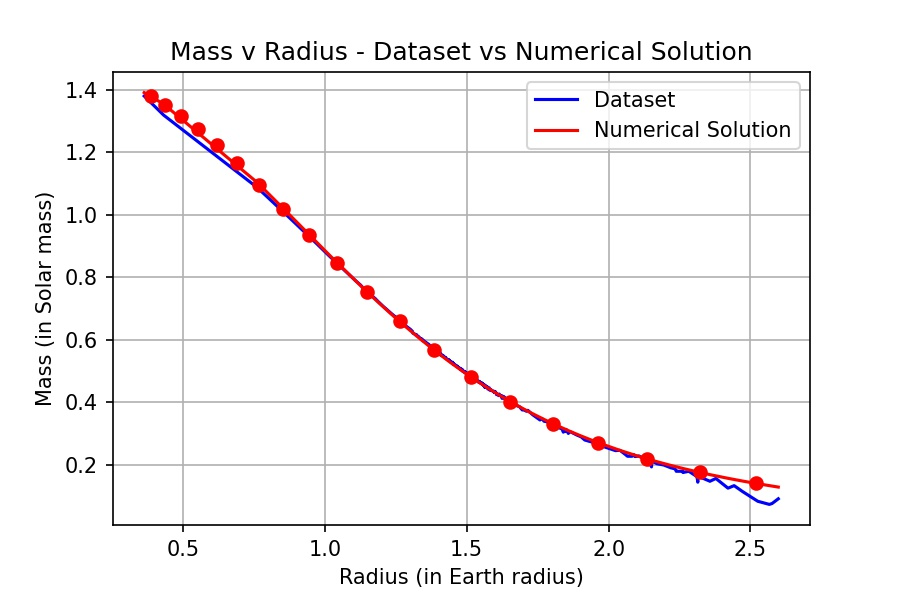
\includegraphics[width=0.85\textwidth]{WD_DatvSol.jpg}
    \caption{Mass v Radius plot, $D=2.00 \times 10^{6}$ fit}
    \end{figure} 
    
\item After plotting a number of $\rho_{c}$ values between $10^{10}$ and $10^{15}$,the White Dwarf mass for which a solution existed was around $1.39M_{\odot}$, which is in accordance with the currently accepted Chandrasekhar limit, $1.4M_{\odot}$. The M-R relationship can be seen in Figure 6.
    
    \begin{figure}[H] 
    \centering
    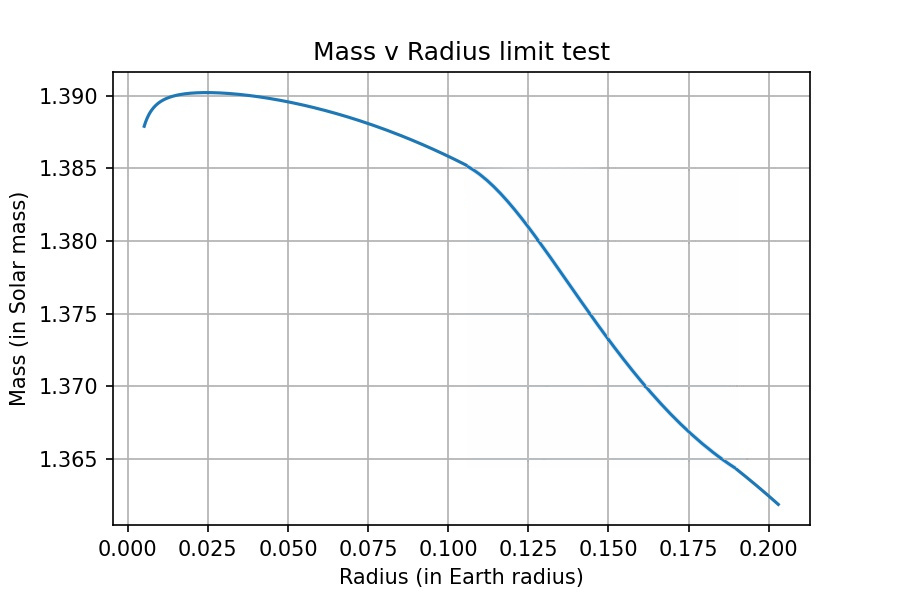
\includegraphics[width=0.85\textwidth]{WD_limit.jpg}
    \caption{Mass v Radius plot for various $\rho_{c}$ values.}
    \end{figure}      



\section{Einstein}

    \begin{enumerate}[label=(\alph*)]
        \item The mass-radius curve for NSs is presented in Figure 7.
        \begin{figure}[H] 
        \centering
        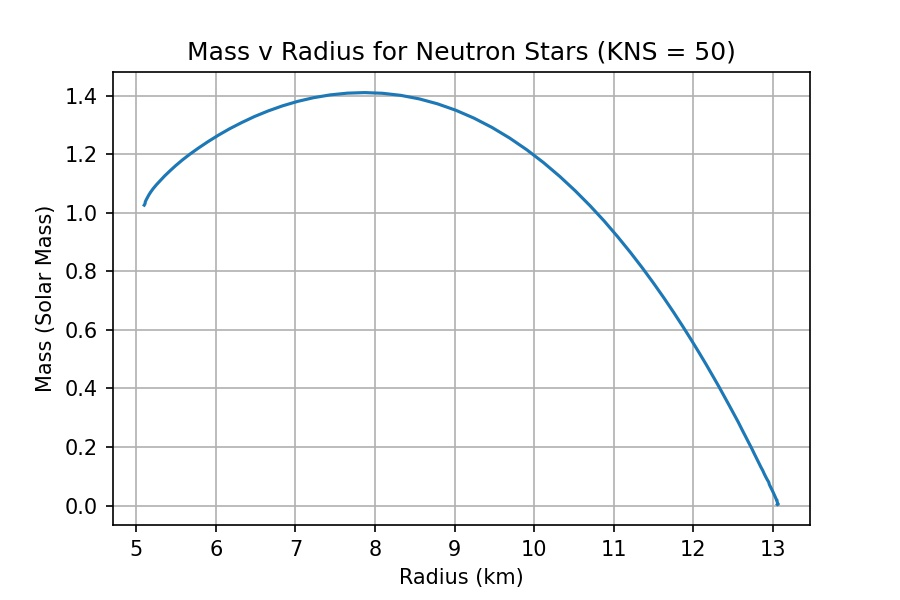
\includegraphics[width=0.85\textwidth]{NS_DatvPrd_50.jpg}
        \caption{M-R plot for neutron stars with $K_{NS} = 50$.}
        \end{figure} 
        
        \item The fractional binding energy($\Delta$)-radius curve for NSs is presented in Figure 8.
        
        \begin{figure}[H] 
        \centering
        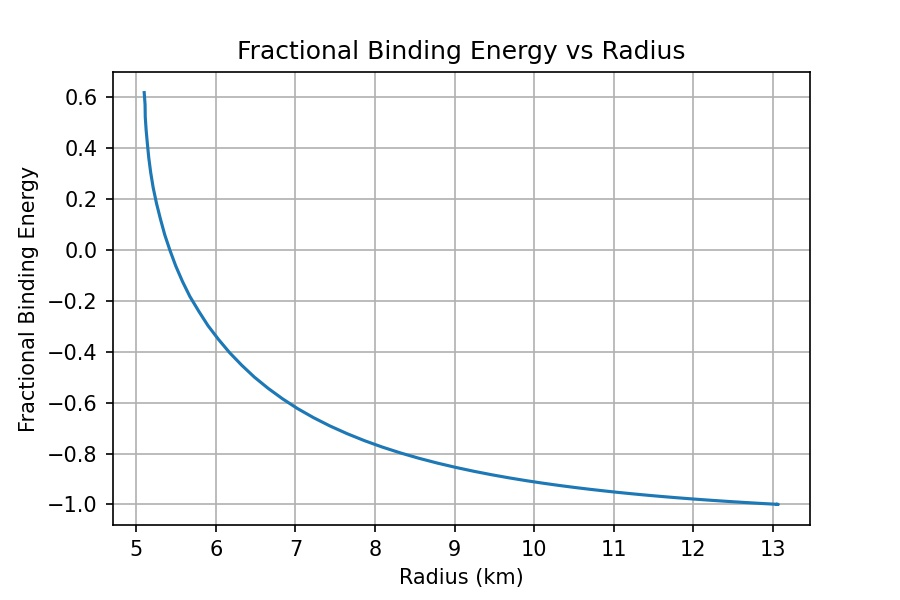
\includegraphics[width=0.85\textwidth]{NS_FBE_50.jpg}
        \caption{$\Delta$-R plot for neutron stars with $K_{NS} = 50$.}
        \end{figure}         
        
        \item The mass-central density($\rho_{c}$) curve for NSs is presented in Figure 9. The maximum stable mass for which the solution exists is $1.41M_{\odot}$, coinciding with $K_{NS} = 50$.
        
        \begin{figure}[H] 
        \centering
        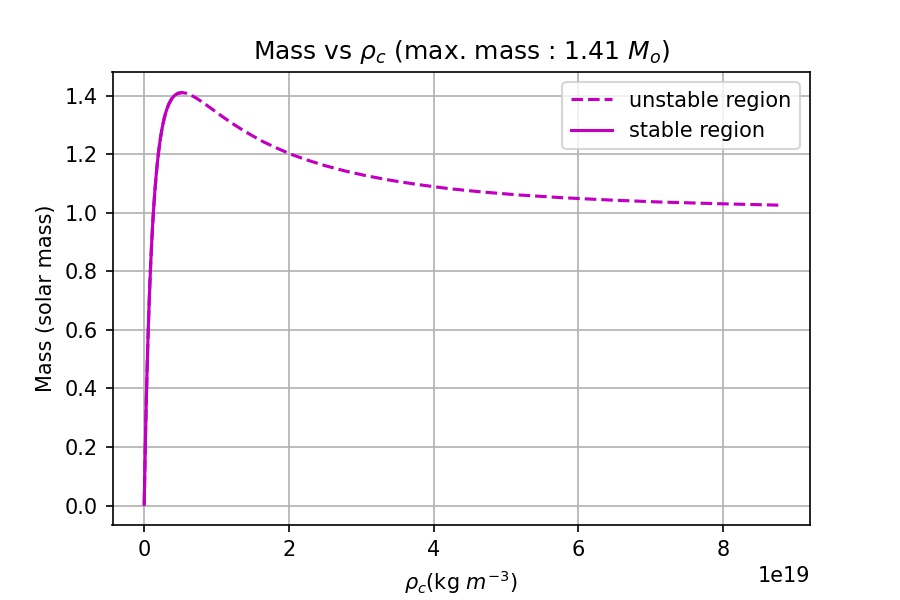
\includegraphics[width=0.85\textwidth]{NS_rho_50.jpg}
        \caption{M-$\rho_{c}$ plot for neutron stars with $K_{NS} = 50$.}
        \end{figure} 
        
        \item The lowest $K_{NS}$ value to have maximum mass greater than $2.14M_{\odot}$, so any $K_{NS}$ is $K_{NS} = 116$, the M and $\Delta-R$ and M-$\rho_{c}$ curves for which are presented in Figures 10, 11, 12. To show another possible value, the graphs for $K_{NS} = 125$ were drawn and presented in Figures 13, 14, 15.
        
        \begin{figure}[H] 
        \centering
        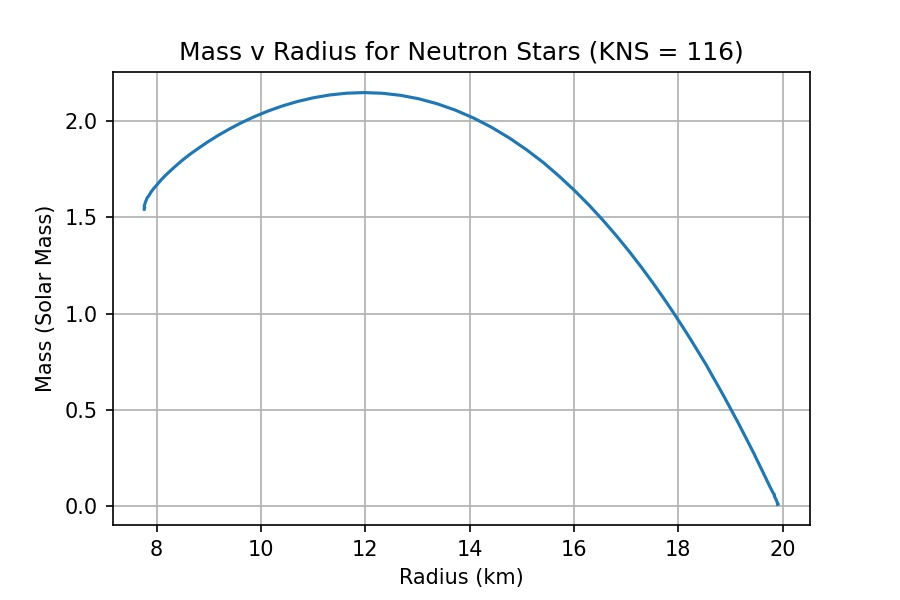
\includegraphics[width=0.85\textwidth]{NS_DatvPrd_116.jpg}
        \caption{M-R plot for neutron stars with $K_{NS} = 116$.}
        \end{figure} 
        
        \begin{figure}[H] 
        \centering
        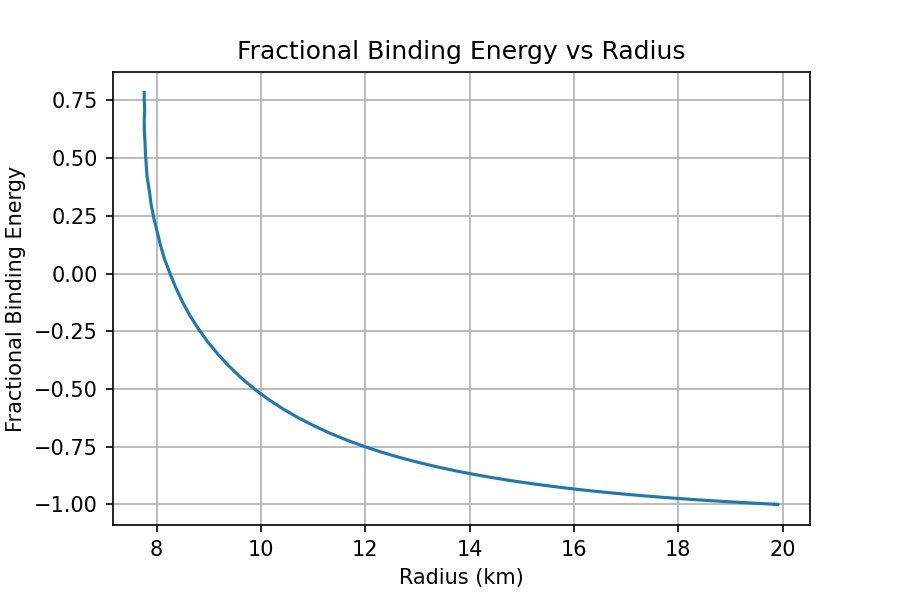
\includegraphics[width=0.85\textwidth]{NS_FBE_116.jpg}
        \caption{$\Delta$-R plot for neutron stars with $K_{NS} = 116$.}
        \end{figure} 
        
        
        \begin{figure}[H] 
        \centering
        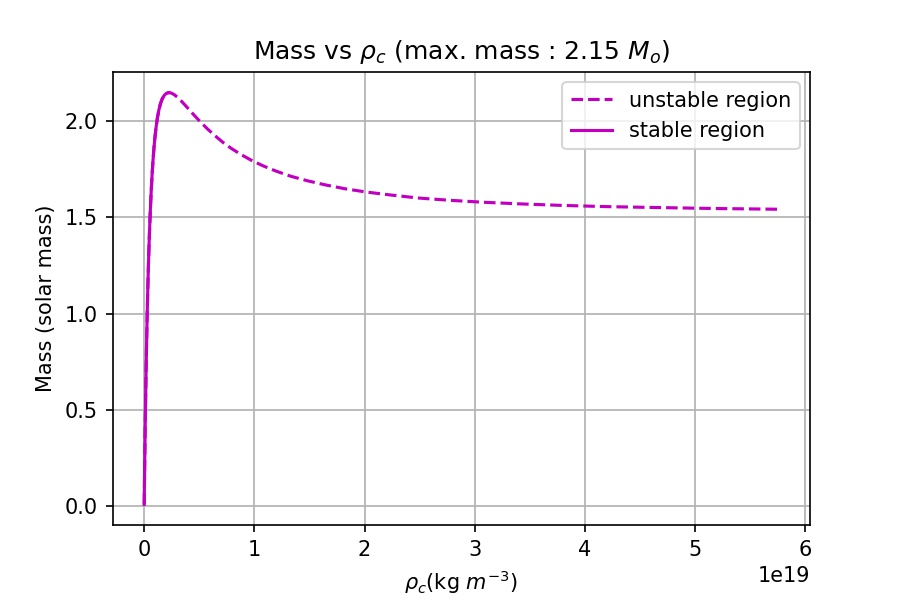
\includegraphics[width=0.85\textwidth]{NS_rho_116.jpg}
        \caption{M-$\rho_{c}$ plot for neutron stars with $K_{NS} = 116$.}
        \end{figure} 
        
        \begin{figure}[H] 
        \centering
        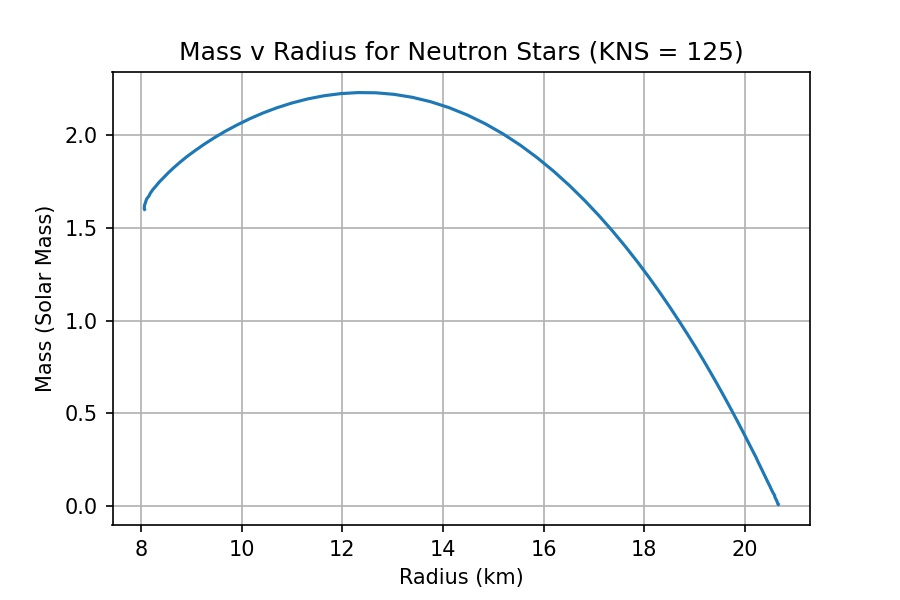
\includegraphics[width=0.85\textwidth]{NS_DatvPrd_125.jpg}
        \caption{M-R plot for neutron stars with $K_{NS} = 125$.}
        \end{figure} 
        
        \begin{figure}[H] 
        \centering
        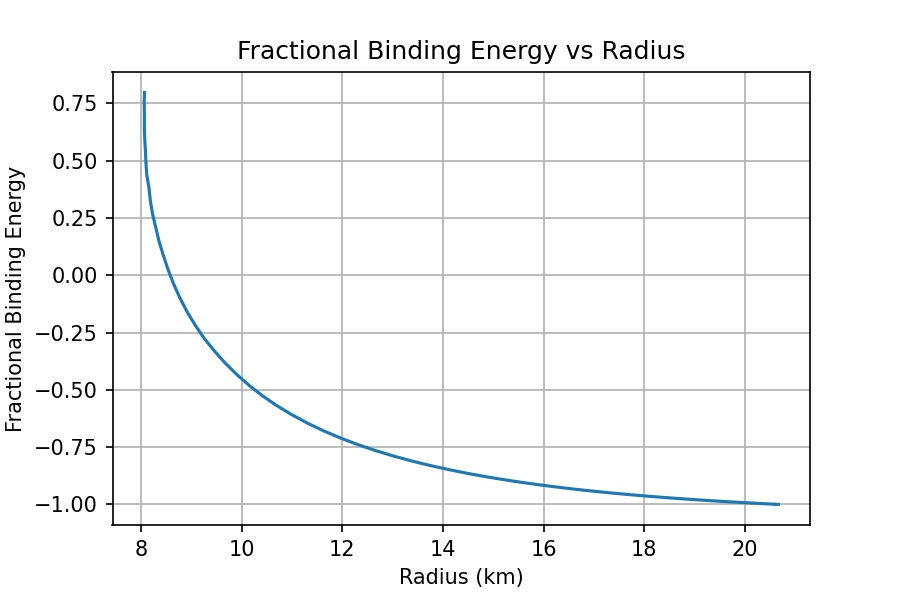
\includegraphics[width=0.85\textwidth]{NS_FBE_125.jpg}
        \caption{$\Delta$-R plot for neutron stars with $K_{NS} = 125$.}
        \end{figure} 
        
        
        \begin{figure}[H] 
        \centering
        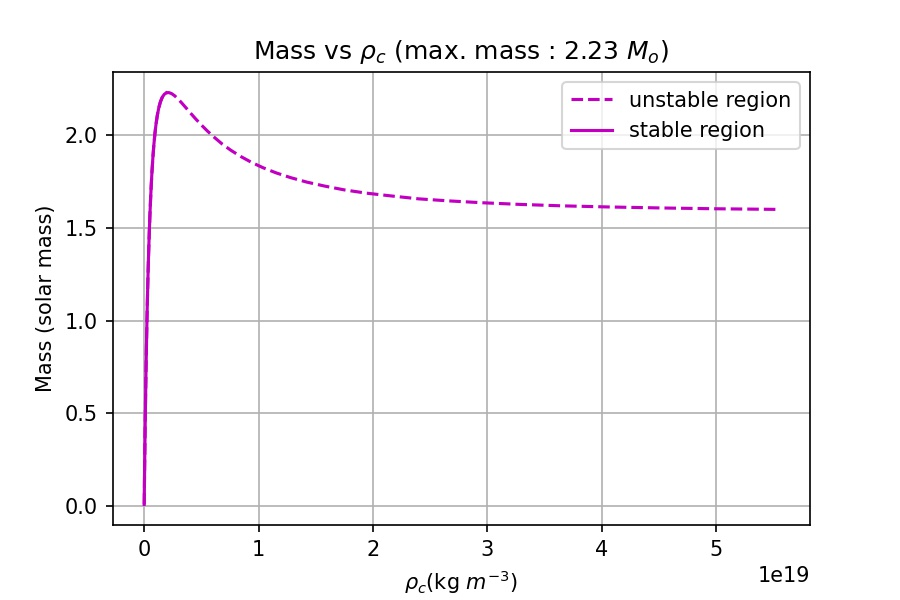
\includegraphics[width=0.85\textwidth]{NS_rho_125.jpg}
        \caption{M-$\rho_{c}$ plot for neutron stars with $K_{NS} = 125$.}
        \end{figure} 
        
        
        \item When $(r > R)$, $\Bar{\nu}(r) = \ln{\left( 1-\frac{2M}{r} \right)}$. Since $\Bar{\nu}(R) = \ln{\left( 1-\frac{2M}{R} \right)}$, adding $\pm \left(\Bar{\nu}(R) - \ln{\left( 1-\frac{2M}{R} \right)}\right)$ would not change the value.
    \end{enumerate}



\end{enumerate}

\end{document}